\documentclass{sig-alternate}

\usepackage{bm}
\usepackage{mathrsfs}
\usepackage{enumerate}
\usepackage[colorlinks=true,linkcolor=cyan]{hyperref}

\usepackage[lined,boxed,ruled,vlined]{algorithm2e}
\SetKwInOut{Input}{Input}
\SetKwInOut{Output}{Output}

\numberofauthors{1}
\author{
\alignauthor
bla
\affaddr{blu} \\
\affaddr{bli}
\email{blo@ble}
}

\newcommand{\va}{\ensuremath{\mathsf{a}}}
\newcommand{\vb}{\ensuremath{\mathsf{b}}}
\newcommand{\vc}{\ensuremath{\mathsf{c}}}
\newcommand{\ve}{\ensuremath{\mathsf{e}}}
\newcommand{\vf}{\ensuremath{\mathsf{f}}}
\newcommand{\vg}{\ensuremath{\mathsf{g}}}
\newcommand{\vh}{\ensuremath{\mathsf{h}}}
\newcommand{\vi}{\ensuremath{\mathsf{i}}}
\newcommand{\vr}{\ensuremath{\mathsf{r}}}
\newcommand{\vu}{\ensuremath{\mathsf{u}}}
\newcommand{\vv}{\ensuremath{\mathsf{v}}}
\newcommand{\vx}{\ensuremath{\mathsf{x}}}
\newcommand{\vy}{\ensuremath{\mathsf{y}}}

\newcommand{\mA}{\ensuremath{\mathsf{A}}}
\newcommand{\mB}{\ensuremath{\mathsf{B}}}
\newcommand{\mC}{\ensuremath{\mathsf{C}}}
\newcommand{\mD}{\ensuremath{\mathsf{D}}}
\newcommand{\mG}{\ensuremath{\mathsf{G}}}
\newcommand{\mH}{\ensuremath{\mathsf{H}}}
\newcommand{\mI}{\ensuremath{\mathsf{I}}}
\newcommand{\mJ}{\ensuremath{\mathsf{J}}}
\newcommand{\mM}{\ensuremath{\mathsf{M}}}
\newcommand{\mN}{\ensuremath{\mathsf{N}}}
\newcommand{\mP}{\ensuremath{\mathsf{P}}}
\newcommand{\mR}{\ensuremath{\mathsf{R}}}
\newcommand{\mS}{\ensuremath{\mathsf{S}}}
\newcommand{\mT}{\ensuremath{\mathsf{T}}}
\newcommand{\mV}{\ensuremath{\mathsf{V}}}
\newcommand{\mW}{\ensuremath{\mathsf{W}}}
\newcommand{\mX}{\ensuremath{\mathsf{X}}}
\newcommand{\mY}{\ensuremath{\mathsf{Y}}}
\newcommand{\mZ}{\ensuremath{\mathsf{Z}}}

\newcommand{\K}{\ensuremath{\mathbb{K}}}
\newcommand{\Q}{\ensuremath{\mathbb{Q}}}
\newcommand{\Z}{\ensuremath{\mathbb{Z}}}

\newcommand{\M}{\ensuremath{\mathscr{M}}}

\newcommand{\lm}{\ensuremath{\operatorname{lm}}}
\newcommand{\rank}{\ensuremath{\operatorname{rank}}}
\newcommand{\DAC}{\ensuremath{\mathsf{DAC}}}
\newcommand{\Iter}{\ensuremath{\mathsf{Iter}}}


\DeclareBoldMathCommand{\bF}{F}
\DeclareBoldMathCommand{\bh}{h}
\DeclareBoldMathCommand{\bu}{u}
\DeclareBoldMathCommand{\bx}{x}
\DeclareBoldMathCommand{\by}{y}

\newcommand{\Otilde}[1]{\ensuremath{O\tilde{~}(#1)}} % soft O for complexity
\newcommand{\todo}[1]{(\textbf{todo:} #1)} 
\newcommand{\why}{\textbf{why?}} 

\newtheorem{pbm}{Problem}
\renewcommand{\thepbm}{\Alph{pbm}} % "letter-numbered" theorems
\newtheorem{definition}{Definition}
\newtheorem{theorem}[definition]{Theorem}
\newtheorem{corollary}[definition]{Corollary}
\newtheorem{proposition}[definition]{Proposition}
\newtheorem{lemma}[definition]{Lemma}
\newtheorem{algo}{Algorithm}

\def\gathen#1{{#1}}

\title{Practical improvements in structured linear algebra}

\begin{document}

\maketitle

\begin{abstract}
bla bla
\end{abstract}

%%%%%%%%%%%%%%%%%%%%%%%%%%%%%%%%%%%%%%%%%%%%%%%%%%%%%%%%%%%%
%%%%%%%%%%%%%%%%%%%%%%%%%%%%%%%%%%%%%%%%%%%%%%%%%%%%%%%%%%%%
%%%%%%%%%%%%%%%%%%%%%%%%%%%%%%%%%%%%%%%%%%%%%%%%%%%%%%%%%%%%

\section{Introduction}

In this paper, we discuss linear algebra algorithms inspired by the
following kind of question: given polynomials such as
\begin{align*}
t_0 &= 8x^4 - 8x^2 + 1\\
t_1 &= 16x^5 - 20x^3 + 5x\\
t_2 &= 32x^6 - 48x^4 + 18x^2 - 1,
\end{align*}
find that the relation $t_0-2x t_1+t_2=0$ holds (this is the
recurrence between Chebyshev polynomials of the first kind).  

More precisely, given input polynomials $(t_0,\dots,t_{s-1})$ over a
field $\K$, together with integers $(n_0,\dots,n_{s-1})$ and $\sigma$,
the {\em Hermite-Pad\'e} approximation problem asks to compute
polynomials $(p_0,\dots,p_{s-1})$, not all zero, such that $\deg(p_i)
< n_i$ holds for all $i$, and such that we have $p_0 t_0 + \cdots +
p_{s-1} t_{s-1}=O(x^\sigma)$. There exist numerous applications to
this type of question, very important particular cases being {\em
  algebraic approximants} (with $t_i =f^i$, for some given $f$) or
{\em differential approximants} (with $t_i =d^if/dx^i$, for some given
$f$); see for instance~\cite[Chapitre~7]{BoChGiLeLeSaSc17}.

Expressed in the canonical monomial bases, the matrix of a
Hermite-Pad\'e problem has size $\sigma \times (n_0 + \cdots +
n_{s-1})$, and consists of $s$ lower triangular Toeplitz blocks. More
generally, our goal in this paper is to compute efficiently elements
in the kernel of {\em mosaic Toeplitz} matrices~\cite{HeAm88}, that
is, $m \times n$ matrices $\mA=(\mA_{i,j})_{1 \le i \le p,1 \le j \le
  q}$ with a $p \times q$ block structure, each of the $pq$ blocks $\mA_{i,j}$
being Toeplitz.

An $m \times n$ Toeplitz matrix $\mA=(a_{i-j})_{1\le i \le m, 1 \le j
  \le n}$ can be succinctly represented by the polynomial
$P_\mA=a_{-n+1} + a_{-n+2} x + \cdots + a_{m-1} x^{m+n-2}$;
multiplication of $\mA$ by a vector $\vb=[b_0~\cdots~b_{n-1}]^t$
amounts to computing $P_\mA P_\vb \bmod x^{m+n-1}$ and keeping the
coefficients of degrees $n-1,\dots,m+n-2$, where we write $P_\vb=b_0 +
\cdots + b_{n-1} x^{n-1}$.  More generally, a mosaic Toeplitz
$\mA=(\mA_{i,j})_{1 \le i \le p,1 \le j \le q}$ can be described by a
sequence of $pq$ such polynomials $\mathscr{P}=(P_{\mA_{i,j}})_{1 \le
  i \le p,1 \le j \le q}$, together with the sequences
$I=(m_1,\dots,m_p)$ and $J=(n_1,\dots,n_q)$ giving the row-sizes,
resp.\ column-sizes of the blocks. Then, our main problem is the
following.

\begin{pbm}\label{pb:mosaic}
  Given polynomials $\mathscr{P}$ and integers $I,J$ as above, 
  defining a mosaic Toeplitz matrix $\mA$, find a non-zero
  vector in the kernel of $\mA$.
\end{pbm}
We consider two situations, first over an arbitrary field $\K$,
counting all operations in $\K$ at unit cost (this is a good model for
computations over finite fields), then specifically over $\Q$, taking
bit-size into account. In all this paper, we closely follow the
existing formalism of {\em structured matrix computations}. In
addition to two new algorithms that complement previous work on the
subject, our main contribution is a discussion on the design and
practical performance of a C++ implementation of some of these
structured matrix algorithms. Our goal being to obtain an
implementation with the best possible performance, a significant part
of the paper is dedicated to e.g. constant time improvements that are 
crucial in practice.

%%%%%%%%%%%%%%%%%%%%%%%%%%%%%%%%%%%%%%%%%%%%%%%%%%%%%%%%%%%%
%%%%%%%%%%%%%%%%%%%%%%%%%%%%%%%%%%%%%%%%%%%%%%%%%%%%%%%%%%%%
%%%%%%%%%%%%%%%%%%%%%%%%%%%%%%%%%%%%%%%%%%%%%%%%%%%%%%%%%%%%

\section{Basics on structured linear algebra}\label{sec:basics}

This section reviews background material on structured matrices; for a
more comprehensive treatment, we refer the reader to~\cite{Pan01}.

\smallskip\noindent{\bf \small Overview.}  Initially developed
in~\cite{KaKuMo79}, the {\it displacement operator} associates to
matrix $\mA$ its displacement $\phi(\mA)$, that is, the image of $\mA$
under a \textit{displacement operator}~$\phi$.  Then, we say that
$\mA$ is structured with respect to $\phi$ if $\phi(\mA)$ has a small
rank compared to its size; the rank of $\phi(\mA)$ is called the
\textit{displacement rank} of $\mA$ with respect to $\phi$. A
prominent example is the family of so-called {\em Toeplitz-like}
matrices, which are structured for the Toeplitz displacement operator
\begin{eqnarray*}
  \phi: \mA & \mapsto & \left( \mZ_m \mA - \mA \mZ_n \right) = 
                        (\mA \downarrow) - (\mA \leftarrow)
\end{eqnarray*}
where $\mZ_n \in \K^{n \times n}$ is the matrix with only ones below the
diagonal.  The displacement rank of a Toeplitz matrix for this operator is at
most two; if $\mA$ is a mosaic Toeplitz with a $p \times q$ block structure, its
Toeplitz displacement rank is at most $p+q$.

The key idea of most algorithms for structured matrices is summarized
by Pan's motto~\cite{Pan01}: compress, operate, decompress. Indeed,
for $\mA$ of size $m \times n$ over a field $\K$, if $\phi(\mA)$ has
rank~$\alpha$, it can be represented using few elements through {\it
  $\phi$-generators}, that is, two matrices $(\mG,\mH)$ in $\K^{m\times
  \alpha} \times \K^{n\times \alpha}$, with $\phi(\mA) = \mG \mH^t$.
The main idea behind algorithms for structured matrices is to use 
generators as a compact data structure, involving $\alpha (m+n)$ field
elements instead of $mn$. 

\smallskip\noindent{\bf \small Cauchy-like matrices.}  Beyond the Toeplitz
structure (and the directly related Hankel one), two other important
cases are so-called Vandermonde and Cauchy structures. While the case
of Toeplitz-like matrices was the first one to be studied in detail,
we will actually focus on Cauchy-like matrices, as we will see that
this particular structure is quite convenient to work with.

For a sequence $\vu=(u_1,\dots,u_m)$ in $\K^m$, let $\mD_\vu \in
\K^{m\times m}$ be the diagonal matrix with diagonal entries
$u_1,\dots,u_m$. Then, given $\vu$ as above and $\vv$ in $\K^n$, we will
consider the operator $\nabla_{\vu,\vv}: \mA \in \K^{m\times n} \mapsto \mD_\vu
\mA - \mA \mD_\vv$; {\em Cauchy-like} matrices (with respect to the
choice of $\vu$ and $\vv$) are those matrices $\mA$ for which
$\nabla_{\vu,\vv}(\mA)$ has small rank.

Let $\vu,\vv$ be given and suppose that $u_i \ne v_j$ holds for all
$i,j$. Then, the operator $\nabla_{\vu,\vv}$ is invertible: given
$\nabla_{\vu,\vv}$-generators $(\mG,\mH)$ of length $\alpha$ for $\mA$, we can reconstruct $\mA$ as
\begin{equation}\label{eq:recA}
\mA = \sum_{i=1}^\alpha
\mD_{\vg_i} 
\mC_{\vu,\vv}\,\mD_{\vh_i},\ \ \ 
\mC_{\vu,\vv}=\begin{bmatrix}
\frac 1{u_1-v_1} & \cdots & \frac 1{u_1-v_n}\\
\vdots & & \vdots \\
\frac 1{u_m-v_1} & \cdots & \frac 1{u_m-v_n}
\end{bmatrix}, 
\end{equation}
where $\vg_i$ and $\vh_i$ are the $i$th columns of respectively $\mG$
and~$\mH$, and  matrix $\mC_{\vu,\vv}$ is known as a {\em Cauchy
  matrix}. Remark that we can
equivalently rewrite $\mA$ as
\begin{equation}\label{eq:recA2}
\mA= (\mG \mH^t) \odot \mC_{\vu,\vv},
\end{equation}
where $\odot$ denotes the entrywise product.

We will have to handle submatrices of $\mA$ through their
generators. The fact that $\mD_{\vu}$ and $\mD_{\vv}$ are diagonal
matrices makes this easy (this is one of the aspects in which the
Cauchy structure behaves more simply than the Toeplitz one).  Suppose
that $(\mG,\mH)$ are generators for $\mA$, with respect to the
operator $\nabla_{\vu,\vv}$, and let $\vu_I=(u_i)_{i \in I}$ and
$\vv_J=(v_j)_{j \in J}$ be subsequences of respectively $\vu$ and
$\vv$, corresponding to entries of indices $I$ and $J$. Let
$\mA_{I,J}$ be the submatrix of $\mA$ obtained by keeping rows and
columns of indices respectively in $I$ and $J$, and let
$(\mG_I,\mH_J)$ be the matrices obtained from $(\mG,\mH)$ by
respectively keeping rows of $\mG$ of indices in $I$, and rows of
$\mH$ of indices in $J$. Then, $(\mG_I,\mH_J)$ is a
$\nabla_{\vu_I,\vv_J}$-generator for $\mA_{I,J}$.

Another useful property relates to inverses of Cauchy-like matrices.
If a matrix $\mA \in \K^{n\times n}$ is invertible, and is structured
with respect to an operator $\nabla_{\vu,\vv}$, its inverse is
structured with respect to $\nabla_{\vv,\vu}$: if $\mD_\vu \mA - \mA
\mD_\vv = \mG \mH^t$, one easily deduces that $\mD_\vv \mA^{-1} - \mA^{-1}
\mD_\vu = - (\mA^{-1} \mG) (\mA^{-t} \mH)^t$ where $A^{-t}$ is a shorthand 
for $(A^{-1})^t$.


\smallskip\noindent{\bf \small Algorithms.}  In most the paper, we
give costs in an algebraic model, counting base field operations at
unit cost (in Section~\ref{sec:lifting}, we work over $\Q$ and use 
a boolean model).

We let $\M$ be such that over any ring, polynomials of degree at most
$d$ can be multiplied in $\M(d)$ base ring operations; we also assume
that the super-linearity assumptions of~\cite[Chapter~8]{GaGe13}
hold. Using the Cantor-Kaltofen algorithm~\cite{CaKa91}, we can take
$\M(d)\in O(d \log(d)\log\log(d))$. We let $\omega$ be a feasible
exponent for linear algebra, in the sense that matrices of size $n$
can be multiplied in $O(n^\omega)$ base ring operations over any ring;
the best bound to date is $\omega < 2.38$~\cite{CoWi90, LeGall14}.
The notation $\Otilde{\,}$ indicates that we omit polylogarithmic
terms. Among the linear algebra operations whose cost reduce to matrix
multiplication, we will have to compute rank and rank
profile~\cite{IbMoHu82}.

Matrix-vector multiplication with $\mC_{\vu,\vv}$ reduces to degree
$n$ polynomial interpolation at the points $\vv$ and evaluation at the
points $\vu$. Using fast polynomial evaluation and interpolation, this
can be done in time $O(\M(p')\log(p'))$, with $p'=\max(m,n)$; thus, we
can multiply matrix $\mA$ of~\eqref{eq:recA} by a vector in time
$O(\alpha \M(p')\log(p'))\subset \Otilde{\alpha p'}$.

In~\cite[Theorem~4.7.3]{Pan01}, Pan shows that if the entries of both
$\vu$ and $\vv$ are in {\em geometric progression}, one can reduce the
cost of the matrix-vector multiplication by $\mC_{\vu,\vv}$ to
$O(\M(p'))$, since polynomial evaluation or interpolation at $n$
points in geometric progression can be done in time $O(\M(n))$;
similarly, multiplication by $\mA$ as above takes time
$O(\alpha\M(p'))$.

We propose here a refinement of this idea, that allows us to
save a constant factor in runtime: we require that $\vu$ and $\vv$ be
geometric progressions with {\em the same ratio} $\tau$. Then, the
cauchy matrix $\mC_{\vu,\vv}$ has entries $1/(u_i -
v_j) = 1/(u_1 \tau^{i-1} - v_1 \tau^{j-1})$, so it can be factored as
$$\mC_{\vu,\vv}=\mD_{\tau^{-1}}
\begin{bmatrix}
\frac 1{u_1 - v_1} & \frac 1{u_1 - v_1 \tau} & \cdots & \frac 1{u_1-v_1 \tau^{n-1}}\\
\frac 1{u_1 - v_1 \tau^{-1}}  & \frac 1{u_1 - v_1} & \cdots & \frac 1{u_1-v_1 \tau^{n-2}}\\
\vdots & & \vdots \\
\frac 1{u_1 - v_1 \tau^{1-m}}  & \frac 1{u_1 - v_1 \tau^{2-m}} & \cdots & \frac 1{u_1-v_1 \tau^{n-m}}
\end{bmatrix},$$
where $\mD_{\tau^{-1}}$ is diagonal with entries
$(1,\tau^{-1},\tau^{-2},\dots,\tau^{1-m})$, and where the left-hand matrix
is Toeplitz. In the reconstruction formula~\eqref{eq:recA}, the
diagonal matrix $\mD_\tau$ commutes with all matrices $\mD_{g_i}$, so
we can take it out of the sum. Hence, we replaced $\alpha$ evaluations
/ interpolations at geometric progressions by $\alpha$ product by
Toeplitz matrices, each of which can be done in a single polynomial
multiplication. The cost for a matrix-vector product by $\mA$ remains
$O(\alpha \M(p'))$, but the constant in the big-O is lower: for $m=n$,
using middle product techniques~\cite{HaQuZi04,BoLeSc03,BoSc05}, the
cost goes down from $3\alpha \M(p') +O(\alpha p')$ to $\alpha \M(p')
+O(\alpha p')$. 

If one needs to multiply $\mA$ as above by {\em several} vectors, further
improvements are possible: we mention (without giving details) an algorithm
from~\cite{BoJeSc08,BoJeMoSc16}, which makes it possible to multiply $\mA$ by $\alpha$
vectors in time $O(\alpha^{\omega-1} \M(p'))$ instead of $O(\alpha^2 \M(p'))$,
by reduction to a sequence of polynomial matrix multiplications.

\smallskip\noindent{\bf \small Reduction from mosaic Toeplitz to Cauchy structure.}
 We said that our primary interest lies in mosaic
Toep\-litz matrices. An important insight of Pan~\cite{Pan90} shows
that one can reduce questions about Toeplitz-like matrices to ones
about Cauchy-like matrices (and conversely, if one wishes to), for a
moderate cost overhead.

To a vector $\vu$ in $\K^m$, let us now associate the corresponding Vandermonde
matrices $\mV_\vu, \mW_\vu \in \K^{m \times m}$
$$
\mV_\vu = 
\begin{bmatrix}
  1 & u_1 & \cdots & u_1^{m - 1}\\
  \vdots & \vdots &  & \vdots\\
  1 & u_m & \cdots & u_m^{m - 1}
\end{bmatrix},
\mW_\vu = 
\begin{bmatrix}
  u_1^{m - 1} & \cdots & u_m^{m - 1}\\
  \vdots &  & \vdots\\
  u_1 & \cdots & u_m\\
  1 & \cdots & 1
\end{bmatrix}.
$$
Given $\vu$ as above, $\vv$ in $\K^n$ and $\mA$ be a Toeplitz-like matrix, we
let $\mA' = \mV_\vu\, \mA\, \mW_\vv$ that is Cauchy-like as we will see. The
$\nabla_{\vu,\vv}$-generators of $\mA'$ depend on the $\phi$-generators of $\mA$
so let's start with those. If $\mA=(\mA_{i,j})_{1 \le i \le p,1 \le j \le q}$ is
mosaic Toeplitz of size $m \times n$, with $\mA_{i,j}$ of size $m_i \times n_j$,
we define the following
\begin{itemize}
\item For $1 \le i \le p$, let $\mA_{i,*}$ be the block matrix
  $[\mA_{i,1}~\cdots~\mA_{i,q}]$.  Let $\eta_i$ be the first row of $\mA_{i,*}$,
  shifted left once, let $\eta'_i$ be the last row of $\mA_{i,*}$, and finally
  let $\vh_i=(\eta'_{i-1}-\eta_i)$ (for $i=1$, $\eta'_0$ is the zero vector);
  this is a row-vector of size $n$. If $\ve_{i,n}$ denotes the row-vector of
  dimension $n$ with only a one at index $i$, we also let $\vg_{i}$ be the
  transpose of $\ve_{m_1 + \cdots +m_{i-1}+1,m}$.
  
\item For $1 \le j \le q$, define $\mA_{*,j}$ similarly to $\mA_{i,*}$;
  $\gamma_j$ and $\gamma'_j$ are its first and last columns, with now a downward
  shift for $\gamma'_j$; in addition, their entry of index $m_1 + \cdots + m_j$
  are set to zero. Then, we define $\vg_{p+j}=(\gamma'_{j}-\gamma_{j+1})$ (as
  above, undefined entries are set to zero).  We also let
  $\vh_{p+j}=\ve_{n_1 + \cdots +n_j,n}$.
\end{itemize}
With these definitions, the matrices
$\mG=\left< \vg_1 | \dots | \vg_{p+q} \right>$ and
$\mH= \left<\vh^t_1 | \dots | \vh^t_{p+q} \right>$ are $\phi$-generators of
$\mA$.

Now we conjugate $\mA$ by Vandermonde matrices since those matrices transform
diagonal matrices into displacement matrices; more precisely, we have the
formulae
\[
  \mD_{\vu}  \mV_{\vu} = \mV_{\vu}  \mZ + (\vu^m)^t \, \ve_{m,m}, \quad
  \mW_{\vv}  \mD_{\vv} = \mZ  \mW_{\vv} + (\ve_{1,n})^t \, \vv^n
\]
where $\vu^m = \begin{bmatrix} u_1^m & \cdots & u_n^m \end{bmatrix}$ and the
same for $\vv^n$.

As a
consequence, if $\phi(\mA)=\mG \mH^t$ then
\begin{eqnarray}
  \nabla_{\vu, \vv} \left( \mathsf{A}' \right) & = & \mD_{\vu}  \mV_{\vu} 
  \mathsf{A}  \mW_{\vv} - \mV_{\vu}  \mathsf{A}  \mW_{\vv}  \mD_{\vv} \nonumber \\
  & = & \mV_{\vu}  \left( \mZ  \mathsf{A} - \mathsf{A}  \mZ \right) \mW_{\vv} 
  \label{eq:gentoetogencau}\\
  &   & + (\vu^m)^t \, \ve_{m,m}  \mathsf{A}  \mW_{\vv} 
        - \mV_{\vu}  \mathsf{A}  (\ve_{1,n})^t \, \vv^n . \nonumber 
\end{eqnarray}

This motivates the following definitions

\begin{itemize}
\item For $1 \le i \le p$, let $\vh'_i=\vh_i \mW_\vv$ and also let $\vg'_{i}$ be
  the column of $\mV_\vu$ of index $m_1 + \cdots +m_{i-1}+1$.
  
\item For $1 \le j \le q$, define $\vg'_{p+j} = \mV_\vu \vg_{p+j}$ and also let
  $\vh'_{p+j}$ be the row of index $n_1 + \cdots +n_j$ in $\mW_\vv$.

\item We define $\vg_{p+q+1} = (\vu^m)^t$, and $\vh_{p+q+1}$ as the last row of
  $\mA \mW_\vv$; we also define $\vg_{p+q+2}$ as the first column of
  $-\mV_\vu \mA$, and $\vh_{p+q+2} = \vv^n$.
\end{itemize}

Then it follows from Eq.~(\ref{eq:gentoetogencau}) that the matrix $\mG'$
with columns $\vg'_1,\dots,\vg'_{p+q+2}$, and the matrix $\mH'$ with columns
that are the transpose of $\vh'_1,\dots,\vh'_{p+q+2}$, are
$\nabla_{\vu,\vv}$-generators of $\mA'$.

The bottleneck in the computation of $\mG'$ and $\mH'$ are $p$
left-products by $\mW_\vv$ and $p$ products by $\mV_\vu$.  If all
entries of $\vu$ and $\vv$ are in geometric progression this takes
time $O(p \M(n) + q \M(m))$; whereas $\mA$ has $\phi$-generators of
length $p+q$, the generators $(\mG',\mH')$ have length $p+q+2$.

\smallskip\noindent{\bf \small Regularization.}  In our algorithms for
Cauchy-like matrices, we will assume that input matrix has {\em
  generic rank profile}, that is, that its leading principal minors of
size up to its rank are invertible.  Regularization for structured
matrices was introduced for this purpose by
Kaltofen~\cite{Kaltofen94}, for the Toeplitz structure. In our Cauchy
context, one could apply to $\mA'$ as defined above the regularization
procedure from~\cite[Section~5.6]{Pan01}, which consists in replacing
$\mA'$ by $\mA'' = \mD_\vx \mC_{\va,\vu} \mA' \mC_{\vv,\vb}\mD_\vy$,
for some new vectors $\vx,\va \in \K^m$ and $\vy,\vb \in
\K^n$. Theorem~5.6.2 in~\cite{Pan01} shows that if $\va,\vu$ consist
of $2m$ distinct scalars, and $\vb,\vv$ consist of $2n$ distinct
scalars, then there exists a non-zero polynomial $\Delta$ in the
entries of $\vx$ and $\vy$, of degree at most $p=\min(m,n)$ in each
block of variables, such that the non-vanishing of $\Delta$ implies
that $\mA''$ has generic rank profile (that theorem is stated for
square matrices, but the result holds in the rectangular case as
well).  The downside of this contruction is that it requires to
compute a pair of generators of length $p+q+4$ for $\mA''$, involving
the multiplication of $\mG'$ and $\mH'$ by $\mC_{\va,\vu}$ and
$\mC_{\vv,\vb}$.

We now point out a simpler construction keeping $\mA' = \mV_\vu\, \mA\, \mW_\vv$
as above. Following the proof of~\cite[Theorem~5.6.2]{Pan01}, we can use the
Cauchy-Binet formula to express the minors of $\mA'$ in terms of those of
$\mV_\vu$, $\mA$ and $\mW_\vv$ as follows. Let $i \le {\rm rank}(\mA)$ and let
$I=\{1,\dots,i\}$. The determinant $\delta_i$ of the $i$th leading principal
minor of $\mA'$ is the sum over all $J=\{j_1,\dots,j_i\} \subset \{1,\dots,m\}$
and $K=\{k_1,\dots,k_i\} \subset \{1,\dots,n\}$ of the terms
$\alpha_{I,J}\, \beta_{J,K}\, \gamma_{K,I}$, where $\alpha_{I,J}$ is the
determinant of $(\mV_\vu)_{I,J}$, $\beta_{J,K}$ is the determinant of
$\mA_{J,K}$, and $\gamma_{K,I}$ is the determinant of $(\mW_\vv)_{K,I}$.

Let $<$ be the monomial ordering on the variables $u_1,\dots,u_i$,
$v_1,\dots,v_i$ that first sorts monomials using the lexicographic order on
$u_1,\dots,u_i$ with $u_1 < \dots < u_i$, and then breaks the ties using the
lexicographic order on $v_1,\dots,v_i$ with $v_1 > \dots > v_i$. If
$J=\{j_1,\dots,j_i\}$ with $j_1 < \dots < j_i$ then the leading monomial
(denoted $\lm(\cdot)$) of $\alpha_{I,J}$ is
$\vu^J := u_1^{j_1-1} \cdots u_i^{j_i-1}$.  Similarly if $K=\{k_1,\dots,k_i\}$
with $k_1 < \cdots < k_i$, then
$\vv^K := v_1^{n-k_1} \cdots v_i^{n-k_i}=\lm(\gamma_{K,I})$. Since $\mA$ is of
rank greater of equal to $i$, at least one of its $i$th minor $\beta_{J,K}$ does
not vanish. Let $J_{\max},K_{\max}$ be the pair of subsets that maximizes
$\vu^J \vv^K$ amongst those for which $\beta_{J,K} \neq 0$. Then we must have
$\lm(\det(\mA'_{I,I})) = \vu^{J_{\max}} \vv^{K_{\max}}$, which shows that
$\det(\mA'_{I,I})$ is non-zero. Note that the partial degrees in all variables
of $\det(\mA'_{I,I})$ is at most $\max(n,m)$. This construction is clearly
favorable since it involves no extra computation on $\mA'$.

\todo{See if we can derive anything for geometric sequences $\vu, \vv$ with the
  same ratio}

%%%%%%%%%%%%%%%%%%%%%%%%%%%%%%%%%%%%%%%%%%%%%%%%%%%%%%%%%%%%
%%%%%%%%%%%%%%%%%%%%%%%%%%%%%%%%%%%%%%%%%%%%%%%%%%%%%%%%%%%%
%%%%%%%%%%%%%%%%%%%%%%%%%%%%%%%%%%%%%%%%%%%%%%%%%%%%%%%%%%%%

\section{Over an abstract field}

In this section, we work over an arbitrary field $\K$, and we explain
how to solve Problem~\ref{pb:mosaic} by using Pan's reduction to the
Cauchy-like Problem~\ref{pb:cauchy} below; this latter task, involving
a Cauchy-like system, will occupy most of the section.

Even though our goal is to solve a linear system, the algorithms do
slightly more: they compute the inverse of a given matrix (or of a
maximal minor thereof); this is similar to what happens for dense
matrices, where we do not know how to solve linear systems with an
exponent better than $\omega$.

We can then state the main question of this section; remark that the
assumptions on the vectors $\vu,\vv$ are slightly stronger than the one
required for $\nabla_{\vu,\vv}$ to be invertible.
\begin{pbm}\label{pb:cauchy}
  Consider vectors $\vu=(u_1,\dots,u_m)$ and $\vv=(v_1,\dots,v_n)$,
  such that $(\vu,\vv)$ has distinct entries. Given
  $\nabla_{\vu,\vv}$-generators of length $\alpha$ for a matrix $\mA$
  in $\K^{m \times n}$, with $\alpha \le \min(m,n)$, do the following:
  \begin{itemize}
  \item if $\mA$ does not have generic rank profile, raise an error,
  \item else, return $\nabla_{\vv',\vu'}$-generators for the inverse
    of the leading principal minor of $\mA$ of order $r$, with
    $\vv'=(v_1,\dots,v_r)$ and $\vu'=(u_1,\dots,u_r)$, where
    $r={\rm rank}(\mA)$.
\end{itemize}
\end{pbm}
There exist two major classes of algorithms for handling such
problems, iterative ones, of cost that grows like $mn$ (for fixed
$\alpha$), and algorithms using divide-and-conquer techniques, of
quasi-linear cost in $m+n$. We stress that having a fast
quadratic-time algorithm is actually crucial in practice: as is the
case for the Half-GCD, fast linear algebra algorithms, etc, the
quasi-linear algorithm will fall back on the quadratic one for input
sizes under a certain threshold, and the performance of the latter
will be an important factor in the overall runtime.

%%%%%%%%%%%%%%%%%%%%%%%%%%%%%%%%%%%%%%%%%%%%%%%%%%%%%%%%%%%%

\subsection{Previous results}

Iterative algorithms that solve a size $n$ Toeplitz system in time
$O(n^2)$ have been known for
decades~\cite{Levinson47,Durbin60,Trench64}; extensions to
structured matrices were later given, as for instance
in~\cite{KaGoOl95}. For the particular form of our
Problem~\ref{pb:cauchy}, we give in Section~\ref{ssec:quad} an
algorithm inspired by~\cite[Algorithme~4]{Mouilleron08}. In this
reference, Mouilleron sketches an algorithm that solves
Problem~\ref{pb:cauchy} in time $O(\alpha n^2)$, in the case where
$m=n$ and $\mA$ is invertible (but without the rank profile
assumption); he credits the origin of this algorithm to
Kailath~\cite[\S1.10]{KaSa99}, who dealt with symmetric matrices.
Our algorithm follows the same pattern, but reduces the cost to 
$O(\alpha^{\omega-2} n^2)$.

In Section~\ref{ssec:MBA-C}, we review divide-and-conquer
techniques. Kaltofen~\cite{Kaltofen94} gave a divide-and-conquer
algorithm that solves the analogue of Problem~\ref{pb:cauchy} for
Toeplitz-like matrices, lifting assumptions of (strong)
non-singularity needed in the original Morf and Bitmead-Anderson
algorithm~\cite{Morf80,BiAn80}; a generalization of his algorithm to
most usual structures is in~\cite{Pan01}.  A further improvement due
to Jeannerod and Mouilleron~\cite{JeMo10}, following Cardinal's
work~\cite{Cardinal99}, allows one to bypass costly ``compression''
stages that were needed in Kaltofen's algorithm and its extensions, by
predicting the shape of the generators we have to compute. For the
case of square Cauchy-like matrices of size $n$, this results in an
algorithm of cost $O(\alpha^2 \M(n)\log(n)^2)$; as pointed out
in~\cite{xxx}, the cost can be reduced to $O(\alpha^2 \M(n)\log(n))$
by choosing vectors $\vu$ and $\vv$ adequately.


%%%%%%%%%%%%%%%%%%%%%%%%%%%%%%%%%%%%%%%%%%%%%%%%%%%%%%%%%%%%

\subsection{Cauchy generators of the inverse}\label{ssec:genofinv}

Let $(\mG,\mH) \in \K^{m\times \alpha} \times \K^{n\times \alpha}$ be
$\nabla_{\vu,\vv}$-generators of a matrix $\mA$ with respect to the
operator $\nabla_{\vu,\vv}$, with $\vu=(u_1,\dots,u_m)$ and
$\vv=(v_1,\dots,v_n)$. Let further $r$ be the rank of $\mA$. Our goal
is to decide if $\mA$ has generic rank profile, and if so, to return
generators $(\mY,\mZ) \in \K^{r\times \alpha} \times \K^{r\times
  \alpha}$ of the inverse of the leading principal minor of $\mA$.


Let $p=\min(m,n)$. For $i$ in $\{0,\dots,p\}$, write $\mA$ as
$$
\mA=\begin{bmatrix}
    \mA^{(i)}_{0,0} & \mA^{(i)}_{0,1} \\[1mm]
    \mA^{(i)}_{1,0} & \mA^{(i)}_{1,1}
  \end{bmatrix}.
$$ 
If the principal minor
 ${\mA^{(i)}_{0,0}}$  is invertible, we define as in~\cite{Cardinal99}
$$
\mS^{(i)} = \begin{bmatrix} 
   {\mA^{(i)}_{0,0}}{}^{-1} &  -{\mA^{(i)}_{0,0}}{}^{-1} \mA^{(i)}_{0,1} \\[1mm]
    \mA^{(i)}_{1,0} {\mA^{(i)}_{0,0}}{}^{-1} & 
    \mA^{(i)}_{1,1} - \mA^{(i)}_{1,0} {\mA^{(i)}_{0,0}}{}^{-1} \mA^{(i)}_{0,1}
\end{bmatrix}.
$$
We see that $( \mS^{(i)})_{i=0\dots p}$ form a sequence of matrix starting from
$\mA$ and ending at $\mA^{-1}$, at least when $\mA$ is square and invertible. To
understand where these matrices come from, let's introduce the matrix
$ \mR^{(0)} = \begin{bmatrix}
  \mA\\
  \mI_{p, n}
\end{bmatrix} = \begin{bmatrix}
  \mS^{(0)}\\
  \mI_{p, n}
\end{bmatrix}
$
in $\K^{(m + p) \times n} $, where $\mI_{p, n} \in \K^{p \times n}$ is
the rectangular matrix with ones on the diagonal. If one performs
column operations to reduce the first $i$th rows
$\begin{bmatrix} \mA^{(i)}_{0,0} & \mA^{(i)}_{0,1} \end{bmatrix}$ of
$\mR^{(0)}$ to $\begin{bmatrix} \mI_{i,i} & 0 \end{bmatrix}$, we get
\begin{equation}\label{eq:Ri}
\mR^{(i)}\!=\!\begin{bmatrix}
     \mI_{i,i} & 0\\
     \mS^{(i)}_{1,0} & \mS^{(i)}_{1,1}\\
     \mS^{(i)}_{0,0} & \mS^{(i)}_{0,1}\\
     0 & \mI_{p - i, n - i}
   \end{bmatrix}\!= \mR^{(0)} \begin{bmatrix}
     \mA_{0, 0}^{(i)} \phantom{}^{- 1} & - \mA_{0, 0}^{(i)} \phantom{}^{- 1} \mA_{0,
     1}^{(i)}\\
     0 & \mI_{n - i,n-i}
   \end{bmatrix}
\end{equation}
A key result for the sequel is~\cite[Proposition~1]{Cardinal99} which states the
Cauchy structure of $\mS^{(i)}$ and gives formulae for its generators. Given
integers $a,b$, $\vu_{a:b}$ denotes the sequence $(u_a,\dots,u_b)$ (and
similarly for $\vv_{a:b}$); we then define $\vu^{(i)}=(\vv_{1:i},\vu_{i+1:m})$
and $\vv^{(i)}=(\vu_{1:i},\vv_{i+1:n})$. Then the matrix $\mS^{(i)}$ is
Cauchy-like for the vectors $\vu^{(i)}, \vv^{(i)}$ ; remark that the operator
$\nabla_{\vu^{(i)},\vv^{(i)}}$ is invertible, in view of our assumption on $\vu$
and $\vv$. Define the $\nabla_{\vu^{(i)},\vv^{(i)}}$-generators
$(\mY^{(i)}, \mZ^{(i)})$ of $\mS^{(i)}$ by decomposing
\[
 \mG=\begin{bmatrix} 
   \mG^{(i)}_0 \\ \mG^{(i)}_1
  \end{bmatrix},\ 
  \mH=\begin{bmatrix} 
        \mH^{(i)}_0 \\    \mH^{(i)}_1 
  \end{bmatrix},\ 
 \mY^{(i)}
 = \begin{bmatrix}
  \mY^{(i)}_0 \\    \mY^{(i)}_1 
     \end{bmatrix},\ 
\mZ^{(i)}
 = \begin{bmatrix}
  \mZ^{(i)}_0 \\    \mZ^{(i)}_1 
     \end{bmatrix},
\]
with $\mG^{(i)}_0, \mH^{(i)}_0, \mY^{(i)}_0, \mZ^{(i)}_0 \in \K^{i \times \alpha}$ such that
\begin{align}
\mY^{(i)}_0&= -{\mA^{(i)}_{0,0}}{}^{-1} \mG^{(i)}_0,\  
&\mY^{(i)}_1&=-\mA^{(i)}_{1,0}{\mA^{(i)}_{0,0}}{}^{-1}\mG^{(i)}_0 + \mG^{(i)}_1,\label{eq:defYi}\\
\mZ^{(i)}_0&= {\mA^{(i)}_{0,0}}^{-t} \mH^{(i)}_0,\  
&\mZ^{(i)}_1&=-{\mA^{(i)}_{0,1}}{}^t{\mA^{(i)}_{0,0}}{}^{-t}\mH^{(i)}_0 + \mH^{(i)}_1\label{eq:defZi}.
\end{align}

\begin{lemma}\label{lemma:cpj-cm}
 $(\mY^{(i)},\mZ^{(i)})$ are $\nabla_{\vu^{(i)},\vv^{(i)}}$-generators for $\mS^{(i)}$.
\end{lemma}

For $i=0$, we simply have $\mS^{(0)}=\mA$ and
$(\mY^{(0)},\mZ^{(0)})=(\mG,\mH)$.  If $\mA$ has generic rank profile,
then the above lemma shows that for $r=\rank(\mA)$,
$(\mY^{(r)}_0,\mZ^{(r)}_0)$ are $\nabla_{\vv',\vu'}$-generators for
${\mA^{(r)}_{0,0}}{}^{-1}$, for $\vu',\vv'$ as in
Problem~\ref{pb:cauchy}, so they solve our problem.

Let $i,j$ be non-negative integers with $0 \le i+j \le p$, and
${\mA^{(i)}_{0,0}}$ invertible. Write a block decomposition of $\mS^{(i)}$, $\mY^{(i)}$ and
$\mZ^{(i)}$ as
\begin{equation*}
\mS^{(i)} = \begin{bmatrix} 
\mS^{(i)}_{0,0} & \mS^{(i,j)}_{0,1} & \mS^{(i,j)}_{0,2}\\
\mS^{(i,j)}_{1,0} & \mS^{(i,j)}_{1,1} & \mS^{(i,j)}_{1,2}\\
\mS^{(i,j)}_{2,0} & \mS^{(i,j)}_{2,1} & \mS^{(i,j)}_{2,2}
    \end{bmatrix},  
\mY^{(i)} = 
\begin{bmatrix}
  \mY^{(i)}_0 \\\mY^{(i,j)}_1 \\\mY^{(i,j)}_2
\end{bmatrix},
\mZ^{(i)} = 
\begin{bmatrix}
  \mZ^{(i)}_0 \\\mZ^{(i,j)}_1 \\\mZ^{(i,j)}_2
\end{bmatrix}
\end{equation*}
with $\mS^{(i,j)}_{1,1} \in \K^{j \times j}$ and
$\mY^{(i,j)}_1, \mZ^{(i,j)}_2 \in \K^{j \times \alpha}$ (from this,
the sizes of all blocks can be deduced).

To solve Problem~\ref{pb:cauchy}, we need to detect when $\mA$ has
generic rank profile. By construction, $\mS^{(i,j)}_{1,1}$ is the
Schur complement of ${\mA^{(i)}_{0,0}}$, seen as a submatrix of
$\mA^{(i+j)}_{0,0}$. This implies the following result.

\begin{lemma}\label{lemma:update}
  Assume that $\mA^{(i)}_{0,0}$ is invertible and has generic rank
  profile.
  $\mA^{(i+j)}_{0,0}$ has generic rank profile if and only if
  $\mS^{(i,j)}_{1,1}$ does, and
  ${\rm rank}(\mA^{(i+j)}_{0,0})=i+{\rm rank}(\mS^{(i,j)}_{1,1})$. 
\end{lemma}

An interesting point is that we can derive $R^{(i+j)}$ from $R^{(j)}$
similarly to the previous operation that computes $R^{(i)}$ from
$R^{(0)}$. Let $\bar{\mS}^{(0)}$ be the matrix $\mS^{(i)}$ where the
$i$ first rows are permuted with the next $j$ rows, and the same for
the columns. If we write $\bar{\mS}^{(j)}$ the sequence of matrices
starting from $\bar{\mS}^{(0)}$, a direct calculation shows the
previous claim that $\mS^{(i+j)}$ is equal to $\bar{\mS}^{(j)}$ after
permuting back its rows and columns. Another more intuitive way to
prove this identity is to show that the column operations that reduce
$\begin{bmatrix} \mA^{(i+j)}_{0,0} & \mA^{(i+j)}_{0,1} \end{bmatrix}$
to $\begin{bmatrix} \mI_{i+j,i+j} & 0 \end{bmatrix}$ can be decomposed
in two operations that respectively reduce the first $i$th rows using
$\mA^{(i)}_{0,0}$ as pivot, then the next $j$th rows using
$\mS^{(i,j)}_{1,1}$ as pivot (see Eq.~(\ref{eq:Ri})).

%%%%%%%%%%%%%%%%%%%%%%%%%%%%%%%%%%%%%%%%%%%%%%%%%%%%%%%%%%%%

\subsection{A faster quadratic algorithm}\label{ssec:quad}

\begin{algorithm}[t]
  \LinesNumbered \DontPrintSemicolon
  \caption{Iterative algorithm $\Iter$ for Problem~\ref{pb:cauchy} \label{algo:iter}}

  \Input{Generators $(\mG,\mH)$ of $\mA$ and step size $\beta$}
  \Output{$r=\rank(\mA), \mY^{(r)}_0,\mZ^{(r)}_0$ or FAIL }
  % \SetKwFunction{Algorithm}{RDAC} \Algorithm{$A,\mathbf{C},i,N,k$}

  $i=0, \mY^{(0)}=\mG, \mZ^{(0)}=\mH, \bar{r} = p$\;
  \While{$i \neq \bar{r}$}{
    $j = \min (\beta,\bar{r}-i)$\;
    Recover $\mS^{(i,j)}_{1,1}$ from its generators $(\mY^{(i,j)}_1,\mZ^{(i,j)}_1)$\;
    Compute the rank and the rank profile of $\mS^{(i,j)}_{1,1}$\; \label{line:rankprof}
    \If{$\mS^{(i,j)}_{1,1}$ does not have generic rank profile}{
      \Return FAIL\;
    }
    \lIf{$\rank( \mS^{(i,j)}_{1,1})\!<\!j$}{
      $j=\rank( \mS^{(i,j)}_{1,1}), \bar{r}=i+j$}
    Recover the row $\mS^{(i,j)}_{1,\ast}$ and column $\mS^{(i,j)}_{\ast,1}$\; \label{line:rowcol}
    Compute the generators $(\mY^{(i+j)},\mZ^{(i+j)})$ of $\mS^{(i+j)}$\; \label{line:nextgen}
    $i = i + j$\;
  }
  Recover $\mS^{(\bar{r})}$ from its generators $(\mY^{(\bar{r})},\mZ^{(\bar{r})})$\;\label{line:recoverwhole}
  Read in $\mS^{(\bar{r})}$ the Schur complement of $\mA^{(\bar{r})}_{0,0}$ in $\mA$\;
  \lIf{Schur complement is non zero}{\Return FAIL}
  \lElse {\Return $(\bar{r},\mY^{(\bar{r})}_0,\mZ^{(\bar{r})}_0)$}
\end{algorithm}

We describe in Algorithm~\ref{algo:iter} an quadratic iterative
algorithm for Problem~\ref{pb:cauchy}; we will use a step size
$\beta \in \{1,\dots,\alpha\}$, given as a parameter.

Note that the formulae that computes $(\mY^{(i+j)},\mZ^{(i+j)})$ from
$(\mY^{(i)},\mZ^{(i)})$ only involves the matrices that belong to the
row or the column of $\mS^{(i,j)}_{1,1}$. So
Algorithm~\ref{algo:iter}, line~\ref{line:rowcol} recovers the
row $\mS^{(i,j)}_{1,\ast}$ from its
$\nabla_{\vu_{i+1:i+j}, \vv^{(i)}}$-generators
$(\mY^{(i,j)}_1,\mZ^{(i)})$ and the column $\mS^{(i,j)}_{\ast,1}$ from
its $\nabla_{\vu^{(i)},\vv_{i+1:i+j}}$-generators
$(\mY^{(i)},\mZ^{(i,j)}_1)$.

\smallskip\noindent{\bf \small Termination and correction.}
The correction of the algorithm is based on the fact that $\mA$ has
generic rank profile if and only if
$\rank(\mA) = \max\{ r \ |\  \forall \ell \leq r, \det(\mA^{(\ell)}_{0,0}) \neq
0 \}$.

The while loop of the algorithm will find the maximal leading
principal minor of $\mA$ that is non-zero and has generic rank
profile. If at some step $i$, we know that $\mA^{(i)}_{0,0}$ is
invertible and has generic rank profile, we use
Lemma~\ref{lemma:update} to determine if $\mA^{(i+j)}_{0,0}$ has the
same properties.

The while loop exits on one of two conditions that both ensures that
$\bar{r} = \max\{ r \ |\ \forall j \leq r, \det(\mA^{(j)}_{0,0}) \neq
0 \}$.
Either $\rank(\mS^{(i,j)}_{1,1})$ is always $j$, then $i$ will
eventually reach $\bar{r}=p$. Or $\rank(\mS^{(i,j)}_{1,1})<j$ at some
point and after setting $\bar{r}=i+\rank( \mS^{(i,j)}_{1,1})$, we
have $\det(\mA^{(\ell)}_{0,0}) \neq 0$ for all $\ell \leq \bar{r}$
and $\det(\mA^{(\bar{r}+1)}_{0,0}) = 0$, and the while loop exits
right after.

After the while loop, it remains to test if $\rank(\mA) = \bar{r}$
which is done by checking that the Schur complement of
$\mA^{(\bar{r})}_{0,0}$ in $\mA$ is zero.

\smallskip\noindent{\bf \small Complexity.} Computing the rank
profile in line~\ref{line:rankprof} costs $O(\beta^\omega)$.  Using
block matrix multiplication in Eq.~\eqref{eq:recA2}, we see that we
can recover the matrices of line~\ref{line:rowcol} in time
$O(\beta^{\omega-2} \alpha (m+n))$ since $j \le \beta \le \alpha$.  To
compute $\mY^{(i+j)}$ on line~\ref{line:nextgen}, we first compute
$\mS^{(i,j)}_{1,1}{}^{-1} \mY^{(i,j)}_1$ in time
$O(\beta^{\omega-1} \alpha)$; then all other operations take time
$O(\beta^{\omega-2} \alpha m)$.  Similarly, computing $\mZ^{(i+j)}$
takes time $O(\beta^{\omega-2} \alpha n)$.  Recovering the whole
matrix $\mS^{(\bar{r})}$ from its
$\nabla_{\vu^{(\bar{r})},\vv^{(\bar{r})}}$-generators
$(\mY^{(\bar{r})},\mZ^{(\bar{r})})$ is done by means
of~\eqref{eq:recA2} with a cost $O(\alpha^{\omega-2} mn)$ using block
matrix multiplication.

One iteration of the while loop costs
$O(\beta^{\omega-2} \alpha (m+n))$; we iterate $O(p/\beta)$ times, for
a total cost of $O(\beta^{\omega-3} \alpha p(m+n))$, which is
$O(\beta^{\omega-3} \alpha mn)$. This dominates the cost of
line~\ref{line:recoverwhole}, so that the whole running time is
$O(\beta^{\omega-3} \alpha mn)$. The algorithm of~\cite{Mouilleron08}
uses $\beta=1$, for which the cost is $O(\alpha mn)$; choosing
$\beta=\alpha$, we benefit from fast matrix multiplication, as the
cost drops to $O(\alpha^{\omega-2} mn)$, as claimed previously.

%%%%%%%%%%%%%%%%%%%%%%%%%%%%%%%%%%%%%%%%%%%%%%%%%%%%%%%%%%%%

\subsection{The divide-and-conquer algorithm}\label{ssec:MBA-C}

\begin{algorithm}[t]
  \LinesNumbered \DontPrintSemicolon
  \caption{Divide-And-Conquer algorithm $\DAC$ \label{algo:dac}}

  \Input{Generators $(\mG,\mH)$ of $\mA$, threshold $t$}
  \Output{$r=\rank(\mA), \mY^{(r)}_0,\mZ^{(r)}_0$ or FAIL }

  $p = \min(m,n), p' = \max(m,n)$\; 

  \lIf{$p' \leq t$}{\Return $\Iter(\mG,\mH, \alpha)$} 
  $i = \lceil p/2 \rceil$\;
  $(r_0,\mY^{(r_0)}_0,\mZ^{(r_0)}_0) = \DAC(\mG^{(i)}_0, \mH^{(i)}_0,  t)$\;\label{line:dac0}

  Compute $(\mY^{(r_0)},\mZ^{(r_0)})$ from $(\mY^{(r_0)}_0,\mZ^{(r_0)}_0)$ and $(\mG,\mH)$
  \label{line:recoverfullgen0}\;

  \If{$r_0 < i$}{
    \lIf{$\mY^{(r_0)}_1 \mZ^{(r_0)}_1{}^t \neq 0$}{\Return FAIL}
    \Return $(r_0,\mY^{(r_0)}_0,\mZ^{(r_0)}_0)$ }

  $(r_1,\mY^{(r_0,r_1)}_1,\mZ^{(r_0,r_1)}_1) = \DAC(\mY^{(r_0)}_1,\mZ^{(r_0)}_1, t)$
  \label{line:dac1}\;

  Compute $(\mY^{(r_0+r_1)}_0,\mZ^{(r_0+r_1)}_0)$ from
  $(\mY^{(r_0,r_1)}_1,\mZ^{(r_0,r_1)}_1)$ and
  $(\mY^{(r_0)},\mZ^{(r_0)})$
  \label{line:recoverfullgen1}\;

  \Return $(r_0+r_1,\mY^{(r_0+r_1)}_0,\mZ^{(r_0+r_1)}_0)$
\end{algorithm}


We now review the divide-and-conquer approach to solving
Problem~\ref{pb:cauchy}, and discuss a constant factor improvement for
the case of certain Cauchy-like matrices. 
\todo{and better dependency $\alpha^{\omega-1}$ in $\alpha$ ? Or not new ?}

Our algorithm proceed essentially following~\cite{JeMo10}, with the
minor difference that do not assume $\mA$ invertible, and that we
explicitly check if $\mA$ satisfies the generic rank profile
assumption.

Recursive calls to $\DAC$ on lines~\ref{line:dac0},~\ref{line:dac1} will raise an error if the submatrices are
not in generic position, so we can assume that we are not in that case.

Computations of
lines~\ref{line:recoverfullgen0},~\ref{line:recoverfullgen1} are f the
same essence ; using Eq.~\eqref{eq:defYi} and~\eqref{eq:defZi}, we can
recover the full generators $(\mY^{(i+j)},\mZ^{(i+j)})$ if we know the
generators $(\mY^{(i,j)}_1,\mZ^{(i,j)}_1)$ of the inverse of the
principal minor $\mS^{(i,j)}_{1,1}$ and previous full generators
$(\mY^{(i)},\mZ^{(i)})$.

\todo{Romain : here}

 \bigskip

%%%%%%%%%%%%%%%%

Let $\mA,\mG,\mH,p,r$ be as in the previous subsection, and for $i$ in
$\{0,\dots,p\}$, define
${\mA^{(i)}_{0,0}},\mA^{(i)}_{0,1},\mA^{(i)}_{1,0},\mA^{(i)}_{1,1},\dots$ as before.
The algorithm will compute the rank $r$ of $\mA$, together with
specific generators for the inverse of the leading principal minor
$\mA_{r,0,0}$, namely $\mY^{(r)}_0=-\mA^{(r)}_{0,0}{}^{-1} \mG^{(r)}_0$ and
  $\mZ^{(r)}_0=\mA^{(r)}_{0,0}{}^{-t}\mH^{(r)}_0$, as did the algorithm in the
  previous subsection.

We choose $i$ in $\{0,\dots,p\}$, and we proceed as follows,
essentially following~\cite{JeMo10}, with the minor difference that do
not assume $\mA$ invertible, and that we explicitly check if $\mA$
satisfies the generic rank profile assumption.

\smallskip\noindent{\bf 0.} If $i$ is less than a certain fixed threshold, return the
output of the algorithm of the previous section.

\smallskip\noindent{\bf 1.} Call the algorithm recursively for the
submatrix ${\mA^{(i)}_{0,0}}$, given by its
$\nabla_{\vu_{1:i},\vv_{1:i}}$-generators
$(\mG^{(i)}_0,\mH^{(i)}_0)$. This will raise an error if
${\mA^{(i)}_{0,0}}$ does not have generic rank profile, so we assume
we are not in that case, and that we know $\rho={\rm
  rank}({\mA^{(i)}_{0,0}})$, $\mY^{(\rho)}_0=-\mA^{(\rho)}_{0,0}{}^{-1}
\mG^{(\rho)}_0$ and $\mZ^{(\rho)}_0=\mA^{(\rho)}_{0,0}{}^{-t}\mH^{(\rho)}_0$.

\smallskip\noindent{\bf 2.} Compute $(\mY^{(\rho)}_1,\mZ^{(\rho)}_1)$
using~\eqref{eq:defYi} and~\eqref{eq:defZi}. The dominant cost is that
of computing the products $\mA^{(\rho)}_{1,0} \mY^{(\rho)}_0$ and
$\mA^{(\rho)}_{0,1}{}^t \mZ^{(\rho)}_0$, given the
$\nabla_{\vu_{\rho+1:m},\vv_{1:\rho}}$-generators
$(\mG^{(\rho)}_1,\mH^{(\rho)}_0)$ of $\mA^{(\rho)}_{1,0}$, and the
$\nabla_{\vu_{1:\rho},\vv_{\rho+1:n}}$-generators
$(\mG^{(\rho)}_0,\mH^{(\rho)}_1)$ of $\mA^{(\rho)}_{0,1}$.  We examine this cost
below.

\smallskip\noindent{\bf 3.} If $\rho < i$, test whether the Schur
complement $ \mA^{(\rho)}_{1,1} - \mA^{(\rho)}_{1,0} \mA^{(\rho)}_{0,0}{}^{-1} \mA^{(\rho)}_{0,1}$ vanishes, or
equivalently whether $\mY^{(\rho)}_1\,
\mZ^{(\rho)}_1{}^t = 0$: if so, return $(\mY^{(\rho)}_0,\mZ^{(\rho)}_0)$; else,
raise an error. This is done by finding a minimal set of
independent rows in $\mZ^{(\rho)}_1$ (this takes time $O(\alpha^{\omega-1}
n)$) and multiplying their transposes  by ${\mY^{(\rho)}_1}$ (there are at most
$\alpha$ such rows, so this takes time $O(\alpha^{\omega-1} n)$ as
well).

\smallskip\noindent{\bf 4.} If $\rho=i$, call the algorithm
recursively for the Schur complement $\mA^{(i)}_{1,1} -
\mA^{(i)}_{1,0} {\mA^{(i)}_{0,0}}^{-1} \mA^{(i)}_{0,1}$, given by its
$\nabla_{\vu_{i+1:m},\vv_{i+1:n}}$-generators
$(\mY^{(i)}_1,\mZ^{(i)}_1)$. This will raise an error if $\mA$ does
not have generic rank profile. Else, we obtain the rank $\sigma$ of the
Schur complement, as well as
$\nabla_{\vv_{i+1:i+\sigma},\vu_{i+1:i+\sigma}}$-generators for its
leading principal minor; with our notation, they are
$-\mS^{(i,\sigma)}_{1,1}{}^{-1} \mY^{(i,\sigma)}_1$ and
$\mS^{(i,\sigma)}_{1,1}{}^{-t} \mZ^{(i,\sigma)}_1$.  

\smallskip\noindent{\bf 5.}  We compute and return
$(\mY^{(i+\sigma)}_0,\mZ^{(i+\sigma)}_0)$ using the formulas of
Lemma~\ref{lemma:update}.  This is done by multiplying the above
matrices by respectively $\mS^{(i,\sigma)}_{0,1}$, given through its
$\nabla_{\vu_{i+1:i+\sigma},\vu_{1:i}}$-generator
$(\mY^{(i)}_0,\mZ^{(i,\sigma)}_{1})$, and
$\mS^{(i,\sigma)}_{1,0}{}^t$, given by its
$\nabla_{\vv_{1:i},\vv_{i+1:i+\sigma}}$-genera\-tor
$(\mY^{(i,\sigma)}_1,\mZ^{(i)}_0)$.

\medskip

The bottleneck in this algorithm, at Steps~{\bf 2} and~{\bf 4}, is the
multiplication of a Cauchy-like matrix of size roughly $m \times n$,
given by generators of lengh $\alpha$, by $\alpha$ vectors, either on
the left or on the right. As explained in Section~\ref{sec:basics},
$\vu$ and $\vv$ are chosen as geometric progressions {\em with the
  same ratio}; if this is the case at the top-level, this will remain
the case for all recursive calls; this allows us to reduce the
matrix-vector products by all Cauchy matrices involved here to
Toeplitz matrix-vector products. Choosing $i=\lceil p/2\rceil$
balances the costs of the two recursive calls; as a result, the
overall runtime of the algorithm is $O(\alpha^2 \M(p') \log(p))$.

%%%%%%%%%%%%%%%%%%%%%%%%%%%%%%%%%%%%%%%%%%%%%%%%%%%%%%%%%%%%

\subsection{Experimental results}

We have implemented the algorithms described so far, together with all
subroutines they rely on, in a C++ library available at
\url{gitsomething}. Our implementation is based on Shoup's
NTL~\cite{Shoup95,NTL} version 10.3.0, and is dedicated to word-size
primes (NTL's \texttt{lzz\_p} class). In all that follows, timings are
measured on an Intel i7-4790 CPU with 32 GB RAM; only one thread is
used throughout.

The main building blocks we need are fast polynomial and matrix
computations. NTL already implements very efficient FFT-based
polynomial arithmetic; matrix multiplication over small fields (for $p
< 2^{23}$) is now extremely efficient, comparable to reference
implementations such as FFLAS-FFPACK~\cite{fflas-ffpack}. On top of
this, we implemented a fast polynomial matrix multiplication, that
relies on the cyclotomic TFT of~\cite{ArSc15}.

We first discuss Problem~\ref{pb:cauchy}. Our first tests compare our
new $O(\alpha^{\omega-2} n^2)$ algorithm to the previous one, with
runtime $O(\alpha n^2)$. Except for very small values of $n$, say $n <
50$, for which the behavior fluctuates rapidly, we found that the new
algorithm becomes more efficient for rather small values of $\alpha$:
our crossover points are $\alpha=8$ or $9$ for primes less than
$2^{23}$, and $\alpha=13$ or $14$ for larger word-size primes. The
following graph shows the time ratio between the direct approach and
our algorithm, for $\alpha=30$. We see that for small primes, for
which matrix multiplication is very efficient, our algorithm brings a
substantial improvement.

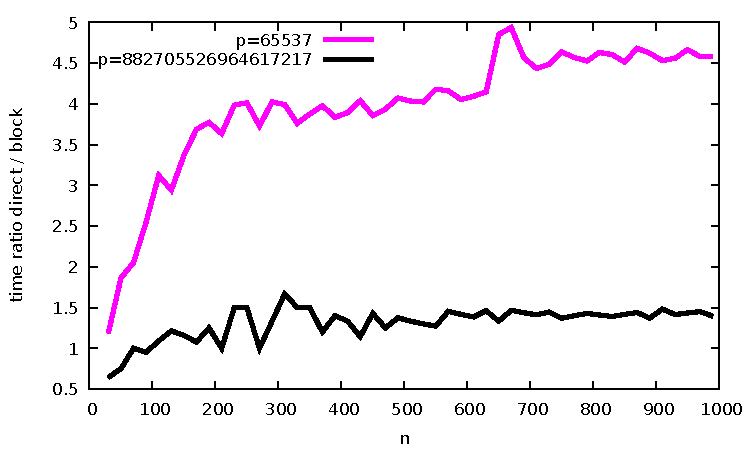
\includegraphics[width=7cm]{ratio-block-eschost-desktop.pdf}

We consider next the divide-and-conquer algorithm. The key factor for
the efficiency of this algorithm is the cost of multiplying an $n
\times n$ Cauchy-like matrix of displacement rank $\alpha$ by an $n
\times \alpha$ dense matrix. We compare here the direct approach of
cost $O(\alpha^2 \M(n))$ to the algorithm of~\cite{BoJeMoSc16}, with
cost $O(\alpha^{\omega-1} \M(n))$, with a view of determining for what
values of $\alpha$ the latter becomes useful. For the former
algorithm, because we are able to cache several forward FFTs, we found
it slightly more advantageous to forego the cyclotomic TFT and simply
use NTL's FFT. As a consequence, the runtime of the first displays the
typical FFT staircaise behavior. This in turn implies that as $n$
grows, the crossover value for $\alpha$ fluctuates, roughly between
$30$ and $55$. The following graph shows the time ratio between then algorithm
of~\cite{BoJeMoSc16} and the direct one, for $\alpha=60$; at
best, the new algorithm wins by a factor of 2. The results do not
depend much on the nature of the prime (since polynomial arithmetic is
a significant part of the runtime, and behaves essentially in the same
manner, independently of $p$).

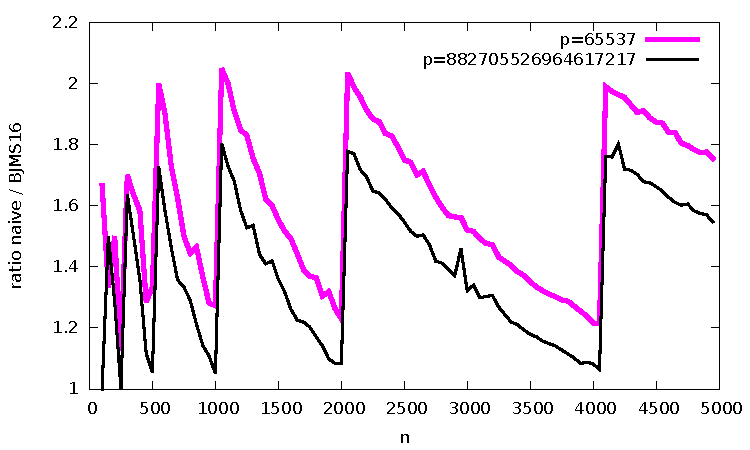
\includegraphics[width=7cm]{ratio-mul-matrix-eschost-desktop.pdf}

Taking these results into account, we determined empirically crossover
values $n_0$ to end the recursion in the divide-and-conquer algorithm,
and switch to the quadratic algorithm. We expect the crossover point
$n_0$ to grow with $\alpha$, since for a given $\alpha$, it behaves
like the solution of $\alpha n^2 = \alpha \M(n) \log(n)$ (assuming
here we do not use fast linear algebra, for simplicity). The following 
table reports some values for $n_0$ (obtained by searching in increments of $100$).
The threshold is higher for small primes, since they benefit more from 
our new quadratic algorithm.

\begin{center}
{\small
\begin{tabular}{|c||c|c|c|c|c|c|c|}\hline
  $\alpha$ & 1 & 5 & 10 & 15 & 20 & 25 &30 \\\hline\hline
$p=65537$  & 400 &400 &500  &1000  &2000  &3300  &4200 \\\hline
$p\simeq 2^{59}$  & 200 & 400 & 400 & 700 & 1300 & 1600 & 2000\\\hline
\end{tabular}
}
\end{center}

These values being set, we can then show runtimes for solving
Problem~\ref{pb:cauchy} modulo both $p=65537$ and
$p=8827055\-26964617217$, for increasing values of $n$; we use
$\alpha=5$, $\alpha=50$ and we also display the runtime of a dense
matrix inversion in the same size. For a very small displacement rank
such as $\alpha=5$, the runtime is essentially the same for these two
primes, since the benefits of fast linear algebra do not
show. However, with $\alpha=50$, we observe a difference, by a factor
of up to 3. In any case, there is a clear gain over dense methods.

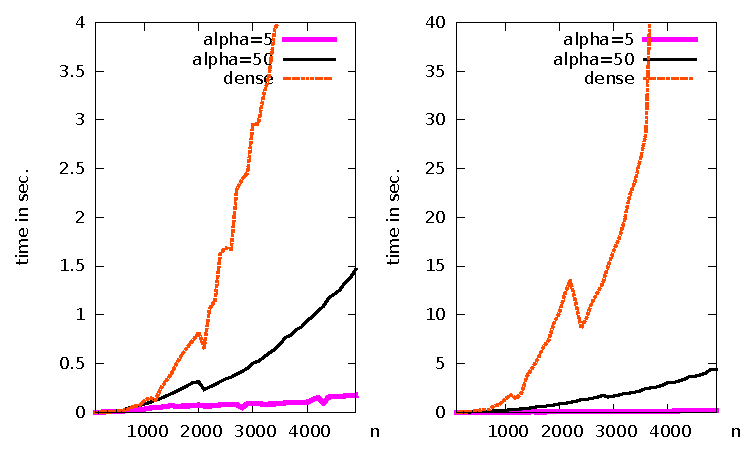
\includegraphics[width=8cm]{large_n-eschost-desktop.pdf}

Our solution of Problem~\ref{pb:mosaic} is a direct reduction to the
Cauchy-like case; we still have to examine the time for putting the
problem into Cauchy form by means of the formulas of~\ref{xxx}.


%%%%%%%%%%%%%%%%%%%%%%%%%%%%%%%%%%%%%%%%%%%%%%%%%%%%%%%%%%%%
%%%%%%%%%%%%%%%%%%%%%%%%%%%%%%%%%%%%%%%%%%%%%%%%%%%%%%%%%%%%
%%%%%%%%%%%%%%%%%%%%%%%%%%%%%%%%%%%%%%%%%%%%%%%%%%%%%%%%%%%%

\section{Modular techniques}\label{sec:lifting}

We now address Problem~\ref{pb:mosaic} in the particular case where
$\K=\Q$; without loss of generality, we assume that the entries of
$\mT$ are integers.

Several {\em modular algorithms} are available to solve dense linear
systems over $\Q$. A first option relies on the Chinese Remainder
Theorem, solving the system modulo several primes $p_1,p_2,\dots$
before reconstructing the solution, making sure to ensure consistency
of the modular solutions when ${\rm ker}(\mT)$ has dimension more than
$1$. Other approaches such as Newton iteration or divide-and-conquer
algorithms use one prime $p$, and lift the solution modulo powers of $p$.

%%%%%%%%%%%%%%%%%%%%%%%%%%%%%%%%%%%%%%%%%%%%%%%%%%%%%%%%%%%%

\subsection{Reduction to nullity one}

Many of these techniques rely on the knowledge of a maximal invertible
minor of $\mA$. However, if $\mA$ is mosaic Toeplitz, there is no
guarantee that it possesses such a minor that would be mosaic Toeplitz
as well. Hence, we are going to rely on the transformation to the
Cauchy structure / regularization technique of~\ref{sec:basics}.
Working over $\Q$, the solution we used before has a certain
shortcoming. Our output is a vector $\vb$ of the form
$\vb=\mW_{\vv}[(-\mA_r^{-1}\vc)^t ~ \vc^t]^t$, with $\mA=\mV_\vu \mT
\mW_{\vv}$, $\mA_r^{-1}$ a maximal minor of it and $\vc$ a random
vector. Due to the preconditionning, the entries of $\vb$ are expected
of large height (the upper bounds one can naively derive from the
formula above seem however to be overly crude).

When ${\rm ker}(\mT)$ has dimension $1$, we are not affected by this
issue. Indeed, in this case, all solutions are of the form $\lambda
\vb_0$, for some vector $\vb_0 \in \Z^n$ whose bit-size can be bounded
only in terms of $\mT$, by an expression in $\Otilde{n h}$, if $h$ is
a bound on the bit-size of the entries of $\mT$ (for instance by means 
of Siegel's lemma). Hence, it suffices to compute the solution $\vb$ 
of the regularized system modulo a large enough integer $N$
and normalize it by setting one of its entries to $1$;
this gives us the normalization of $\vb_0 \bmod N$.

For an arbitrary $\mT$, our suggestion is to reduce to 
nullity $1$ by adding extra rows to $\mT$

In the important particular case of algebraic approximation,
we suggest another method.

%%%%%%%%%%%%%%%%%%%%%%%%%%%%%%%%%%%%%%%%%%%%%%%%%%%%%%%%%%%%

\subsection{The divide-and-conquer algorithm}

%%%%%%%%%%%%%%%%%%%%%%%%%%%%%%%%%%%%%%%%%%%%%%%%%%%%%%%%%%%%

\subsection{The divide-and-conquer algorithm}





\bibliographystyle{plain} {\scriptsize \bibliography{structured}}


\end{document}
